\section{Експеримент}

У овом поглављу описан је експеримент који треба да измери перформансе секвенцијалног, односно паралелног решења.
Такође, представљен је преглед резултата експеримента, то јест, упоредни приказ оба решења.

\subsection{Опис експеримента}

Експеримент описан у овом поглављу треба да измери перформансе секвенцијалног и паралелног решења у различитим случајевима коришћења.

Проблем проналаска суме у бинарном стаблу генерално је веома незахтеван што се тиче процесорских ресурса.
То се дешава због чињенице да је обрада појединачног чвора веома краткотрајна у погледу процесорског времена.
Стога, како би проблем било доследније измерити
\footnote{Приликом иницијалних мерења, оба решења су изузетно брзо долазила до краја извршавања.
Дешавало се да времена извршавања једног решења буду многоструко различита.
То се дешавало због стохастичних процеса попут процесорског кеширања, изборa задатка за извршавање од стране OpenMP библиотеке итд.
који су од извршавања до извршавања били мање или више повољнији.},
у секвенцијално и паралелно решење додато је време обраде појединачног чвора од $1\mu s$.

Природа паралелног решења је таква да су сви OpenMP задаци 

Паралелно решење покретано је са \textbf{8, 4 и 2 процесуирајуће јединице}.
Бројева 8, 4 и 2 су изабрани због тога што су то степени броја два тј. бројеви чворова на нивоима 3, 2 и 1 бинарног стабла, респективно, те ова решења нуде
могућност паралелне обраде $l$ чворова. Међутим, решење је покретано и са 12 ПЈ, јер се при иницијалним мерењима показала предност покретања паралелног решења
и са бројем ПЈ који није умножак двојке, а која се своди на следеће: сви OpenMP задаци у паралелном решењу познати су тек када сви задаци на нивоу $l-1$ започну
своје извршавање и генеришу те задатке; OpenMP извршно окружење фаворизује редно извршавање задатака, онај задатак који се генерише раније, он ће се раније и извршити.
Последица свега овога јесте да 

Решења су покретана над стаблима величина 100 хиљада чворова, 10 хиљада чворова и 9 чворова (пример са слике \ref{fig:primersume}).
Тражена сума је бирана тако да се:
\begin{enumerate}
    \item Nе може доћи до решења.
    \item Сума налази на путањи састављеној од све леве деце-чворова (оптималан случај секвенцијалног решења). Означено као \textbf{решење Л}.
    \item Сума налази на путањи састављеној од деце-чворова биране тако да се наизменично бирају лево и десно дете-чвор (погодан случај паралелног решења).
    Означено је као \textbf{решење С}.
\end{enumerate}

\subsection{Резултати}

\begin{figure}[H]
    \centering
    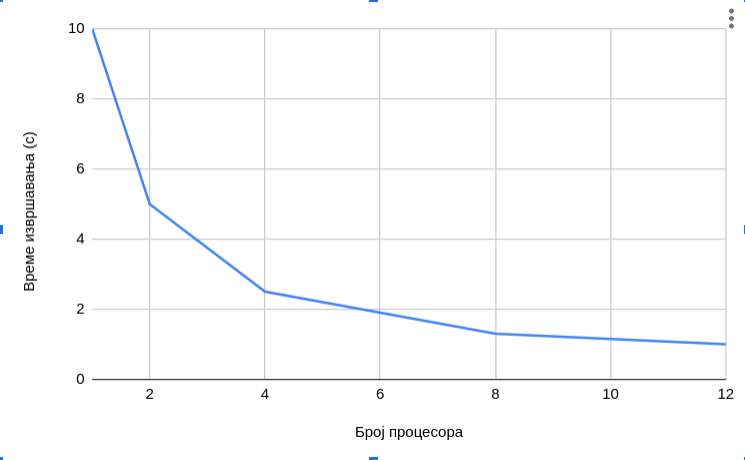
\includegraphics[scale = 0.7]{zavisnost.png}
    \caption{Резултати покретања решења са растућим бројем процесуирајућих јединица}
    \label{fig:rezultati2}
\end{figure}

На слици \ref{fig:rezultati2} приказана је брзина извршавања решења у односу на растући број процесуирајућих јединица.
Секвенцијално решење представљено је подацима о извршавању са 1 процесуирајућом јединицом.
Перформансе извршавања секвенцијалног решења су, наравно, независне од броја процесуирајућих јединица.




\pagebreak